\documentclass[12pt,letterpaper]{article}

\usepackage[spanish,es-tabla,es-nodecimaldot]{babel}
\usepackage{amsmath}
\usepackage[utf8]{inputenc}
\usepackage[T1]{fontenc}
\usepackage{lmodern}
\usepackage{graphicx}
\usepackage{listings}
\usepackage{anysize} 
\usepackage{fancyhdr}
\usepackage{amsmath}
\usepackage{pdfpages}
\usepackage{graphics}
\usepackage{capt-of}
\usepackage{tabularx}
\usepackage{booktabs}
\usepackage[colorlinks=true,plainpages=true,citecolor=blue,linkcolor=blue]{hyperref}

\marginsize{2cm}{2cm}{2cm}{2cm}
\pagestyle{fancy}
\fancyhf{Teoría de la Información}
\fancyhead[L]{\footnotesize UPIITA-IPN} 
\fancyhead[R]{\footnotesize 2TM4} 
\fancyfoot[R]{\footnotesize Práctica 5}
\fancyfoot[C]{\thepage}
\fancyfoot[L]{\footnotesize Reporte} 
\renewcommand{\footrulewidth}{0.4pt}
\renewcommand{\spanishtablename}{Tabla}
\renewcommand{\labelitemii}{$\star$}
\graphicspath{ {C:/Users/Anselmo-PC/Documents/GitHub/upiita-RedesTelecomunicaciones/MemoriaTecnica/imagenes} }

\begin{document}

\includepdf[pages={1}]{portada}
\newpage
\tableofcontents
\listoffigures
\listoftables

\newpage
\section{Objetivo}
Implementación en hardware de un codificador de canal de bloque mediante la utilizacion 
de dispositivos lógicos programables.

\section{Descripción}
A partir de una matriz generadora perteneciente a un CBS(n, k), se implementrán en dispositivo 
programable tanto la parte codificadora (coder) como la parte decodificadora (decoder) de dicho
codificador, de acuerdo con el siguiente diagrama.
\begin{figure}[ht]
    \centering
    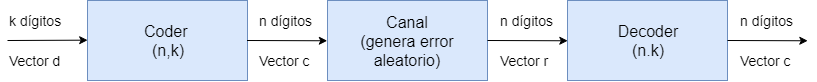
\includegraphics[width=1\textwidth]{d0.png}
    \caption{Daigrama a bloques general del codificador a implementar.}
\end{figure}

\section{Análisis}
\subsection{Palabras código}
A partir de la matriz generadora G y la siguiente ecuación se pueden obtener la palabras código.
\begin{equation}
    c=d G
\end{equation}
Donde:
\begin{itemize}
    \item \textbf{c: } palabra código.
    \item \textbf{d: } palabra doto.
    \item \textbf{G: } matriz generadora.
\end{itemize}
La matriz generadora es la siguiente:
\[
G
=
\begin{bmatrix} 
    0 & 1 & 1 & 1 & 1 & 0 & 0 & 0 \\
    1 & 1 & 1 & 0 & 0 & 1 & 0 & 0 \\
    1 & 1 & 0 & 1 & 0 & 0 & 1 & 0 \\
    1 & 1 & 1 & 1 & 0 & 0 & 0 & 1 \\
    \end{bmatrix}
\]
El vector de la palabra dato es:
\begin{equation}
    \vec{d}=[d_1 \ d_2 \ d_3 \ d_4]
\end{equation}
Realizando la operación se podrán obtener los diferentes valores del vector $\vec{c}$.
Las ecuaciones resultantes de esta operación son las siguientes.
$$c_1=d_2 \bigoplus d_3 \bigoplus d_4$$
$$c_1=d_1 \bigoplus d_2 \bigoplus d_3$$
$$c_1=d_1 \bigoplus d_2 \bigoplus d_4$$
$$c_4=d_1 \bigoplus d_3 \bigoplus d_4$$
$$c_1=d_1$$
$$c_1=d_2$$
$$c_1=d_3$$
$$c_1=d_4$$

Y la palabra código resultante es:
\begin{equation}
    \vec{c}=[c_1 \ c_2 \ c_3 \ c_4 c_5 \ c_6 \ c_7 \ c_8]
\end{equation}

\newpage
A continuación se muestra la tabla con las diferentes para datos con su respectiva palabra 
código.
\begin{table}[ht]
    \centering
    \begin{tabular}{|c|c|c|c|c|c|c|c|c|c|c|c|c|}
    \hline
    %Palabra dato \multicolumn{2}{c}{Var} &  &  &  &  &  &  &  &  &  &  & & \\ \hline
    \multicolumn{3}{c}{Palabra dato } & & \multicolumn{7}{c}{Palabra código}   \\ \hline
    $d_1$ & $d_2$ & $d_3$ & $d_4$ & & $c_1$ & $c_2$ & $c_3$ & $c_4$ & $c_5$ & $c_6$ & $c_7$ & $c_8$ \\ \hline
    0 & 0 & 0 & 0 & & 0 & 0 & 0 & 0 & 0 & 0 & 0 & 0 \\ \hline
    0 & 0 & 0 & 1 & & 1 & 0 & 1 & 1 & 0 & 0 & 0 & 1 \\ \hline
    0 & 0 & 1 & 0 & & 1 & 1 & 0 & 1 & 0 & 0 & 1 & 0 \\ \hline
    0 & 0 & 1 & 1 & & 0 & 1 & 1 & 0 & 0 & 0 & 1 & 1 \\ \hline
    0 & 1 & 0 & 0 & & 1 & 1 & 1 & 0 & 0 & 1 & 0 & 0 \\ \hline
    0 & 1 & 0 & 1 & & 0 & 1 & 0 & 1 & 0 & 1 & 0 & 1 \\ \hline
    0 & 1 & 1 & 0 & & 0 & 0 & 1 & 1 & 0 & 1 & 1 & 0 \\ \hline
    0 & 1 & 1 & 1 & & 1 & 0 & 0 & 0 & 0 & 1 & 1 & 1 \\ \hline
    1 & 0 & 0 & 0 & & 0 & 1 & 1 & 1 & 1 & 0 & 0 & 0 \\ \hline
    1 & 0 & 0 & 1 & & 1 & 1 & 0 & 0 & 1 & 0 & 0 & 1 \\ \hline
    1 & 0 & 1 & 0 & & 1 & 0 & 1 & 0 & 1 & 0 & 1 & 0 \\ \hline
    1 & 0 & 1 & 1 & & 0 & 0 & 0 & 1 & 1 & 0 & 1 & 1 \\ \hline
    1 & 1 & 0 & 0 & & 1 & 0 & 0 & 1 & 1 & 1 & 0 & 0 \\ \hline
    1 & 1 & 0 & 1 & & 0 & 0 & 1 & 0 & 1 & 1 & 0 & 1 \\ \hline
    1 & 1 & 1 & 0 & & 0 & 1 & 0 & 0 & 1 & 1 & 1 & 0 \\ \hline
    1 & 1 & 1 & 1 & & 1 & 1 & 1 & 1 & 1 & 1 & 1 & 1 \\ \hline
    \end{tabular}
    \caption{Palabras dato y código.}
    \label{Palabras dato y código.}
\end{table}



\subsection{Síndrome}
\subsection{Corrección de error}

\newpage
\section{Circuito}

\newpage
\section{Código}

\newpage
\section{Algoritmo}

\newpage
\section{Conclusiones}
\end{document}